\clearpage
\section*{CHƯƠNG 9. TRIỂN KHAI VÀ ĐÁNH GIÁ TRÊN FPGA}
\addcontentsline{toc}{section}{\numberline{}CHƯƠNG . TRIỂN KHAI VÀ ĐÁNH GIÁ TRÊN FPGA}
\setcounter{section}{9}
\setcounter{subsection}{0}
\setcounter{figure}{0}
\setcounter{table}{0}

Chương này trình bày quá trình triển khai và kiểm chứng lõi xử lý mật mã hỗn loạn trên môi trường phần cứng vật lý FPGA. Sau khi thiết kế RTL đã được kiểm chứng chức năng thông qua quá trình mô phỏng, lõi mật mã được tiến hành bọc lại và tích hợp với các phân hệ giao tiếp ngoại vi để truyền nhận dữ liệu trực tiếp với máy tính. Mục tiêu trọng tâm của chương là đánh giá độ ổn định của thiết kế trên bo mạch thực tế, đồng thời đo lường hiệu năng và độ trễ xử lý thông qua một hệ thống bộ đếm chu kỳ phần cứng tích hợp.

\subsection{Mô hình kiểm chứng vòng kín PC--FPGA--PC}

Mô hình kiểm chứng được thiết lập theo kiến trúc vòng lặp khép kín giữa máy tính và bo mạch vi mạch. Trong mô hình này, máy tính đóng vai trò là trạm điều khiển, chịu trách nhiệm sinh chuỗi dữ liệu bản rõ hoặc bản mã, sau đó đóng gói và truyền xuống phần cứng thông qua chuẩn giao tiếp nối tiếp. Tại thiết bị phần cứng, vi mạch sẽ tiếp nhận luồng dữ liệu, tự động phân mảng thành các khối 25 byte và đẩy vào lõi mật mã để xử lý. Kết quả xử lý ngay lập tức được vi mạch truyền ngược về máy tính để phần mềm tiến hành lưu trữ và đối chiếu tính đúng đắn. Phép phương pháp triển khai này cho phép đánh giá chéo trực tiếp hiệu năng giữa phần mềm và phần cứng trong điều kiện hoạt động thời gian thực.

\begin{figure}[H]
	\centering
	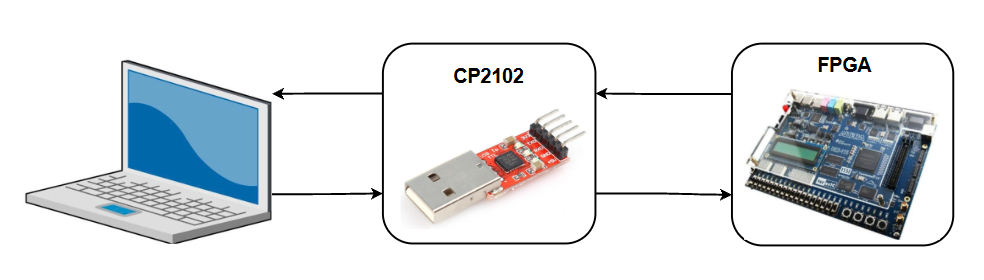
\includegraphics[width=0.8\textwidth]{Figures/flow.png}
	\caption{Mô hình kiểm chứng lõi mật mã trên FPGA thông qua cổng nối tiếp}
	\label{fig:pc_fpga_model}
\end{figure}

\subsection{Thiết kế khối giao tiếp mức cao Board\_Top\_Wrapper}

Để kết nối các module lõi độc lập thành một hệ thống hoàn chỉnh, đồ án xây dựng một khối bao bọc mức cao nhất mang tên \texttt{Board\_Top\_Wrapper}. Khối này hoạt động như một trạm điều phối trung tâm, kết nối lõi mật mã \texttt{crypto\_top} với hệ thống truyền nhận UART và các linh kiện ngoại vi trên bo mạch. Cốt lõi của khối bao bọc này là một máy trạng thái điều phối đa tốc độ. Quá trình vận hành bắt đầu từ việc máy trạng thái chờ nhận đủ 25 byte dữ liệu từ khối nhận UART, sau đó kích hoạt lõi mật mã thực thi. Ngay khi nhận được cờ báo hoàn tất từ hệ thống tính toán, máy trạng thái sẽ chuyển sang luồng truyền dữ liệu, đẩy tuần tự 25 byte kết quả về lại máy tính trước khi khởi động lại vòng lặp cho khối dữ liệu tiếp theo.

Đặc biệt, để đánh giá chính xác độ trễ thực thi của thuật toán, khối bao bọc được tích hợp thêm một hệ thống bộ đếm chu kỳ phần cứng độc lập. Bộ đếm này được thiết kế để bắt đầu tăng giá trị theo xung nhịp 50 MHz ngay khi lõi mật mã được kích hoạt và dừng đếm khi thuật toán hoàn tất. Nhằm khắc phục hiện tượng nhiễu nhấp nháy trên dàn hiển thị, giá trị đếm được thiết kế để chỉ chốt vào thanh ghi đệm \texttt{display\_count} khi toàn bộ một khối dữ liệu đã được xử lý xong. Giá trị trong thanh ghi đệm này sau đó được xuất qua mạch giải mã để hiển thị trực quan kết quả số chu kỳ tiêu tốn lên hệ thống 8 LED 7 thanh trên bo mạch DE2-115.

\subsection{Phần mềm truyền nhận và giao tiếp ngoại vi}

Về mặt kết nối vật lý, đồ án sử dụng một module chuyển đổi USB sang mức điện áp TTL (CP2102) làm cầu nối giữa cổng USB của máy tính và các chân mở rộng của FPGA. Giao tiếp này được đấu nối chéo đường truyền nhận, tạo ra một kênh liên lạc an toàn.

\begin{figure}[H]
	\centering
	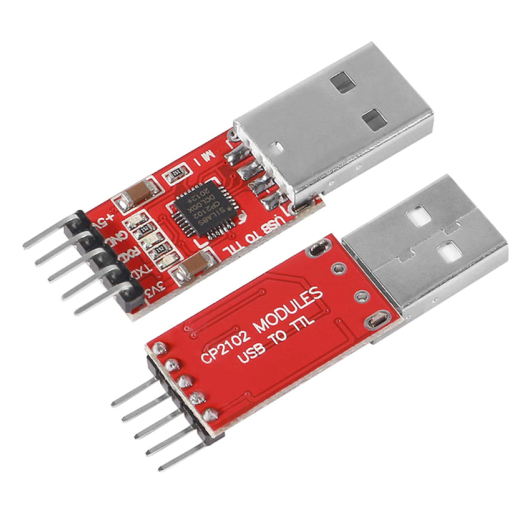
\includegraphics[width=0.3\textwidth]{Figures/cp2102.png}
	\caption{Module chuyển đổi USB--TTL CP2102 sử dụng trong hệ thống}
	\label{fig:cp2102}
\end{figure}

Để tự động hóa luồng đẩy dữ liệu, một kịch bản mã nguồn Python được xây dựng trên máy tính. Phần mềm sẽ mở cổng COM giao tiếp với tốc độ baud được ấn định ở mức 115200 bit/giây. Để đảm bảo đồng bộ phần cứng, kịch bản Python sẽ tự động xả các tín hiệu nhiễu trên đường truyền và dọn dẹp bộ đệm ngay khi vừa mở cổng. Khi đọc dữ liệu từ tệp tin gốc, nếu tổng lượng dữ liệu không chia hết cho 25, phần mềm sẽ tự động chèn thêm các byte mang giá trị 0 vào cuối mảng để lấp đầy khối dữ liệu. Dữ liệu sau đó được phần mềm đẩy trực tiếp xuống vi mạch theo từng khối 25 byte liên tục ở tốc độ cao. Cùng lúc đó, phần mềm sẽ đứng chờ để nhận lại đúng 25 byte kết quả, ghi xuất ra tệp tin đích và tự động đo lường thời gian thực thi của toàn bộ quá trình truyền nhận khối.

\begin{table}[H]
	\centering
	\caption{Kết nối vật lý giữa module CP2102 và vi mạch FPGA}
	\label{tab:uart_connection}
	\renewcommand{\arraystretch}{1.4}
	\begin{tabular}{|l|l|p{6cm}|}
		\hline
		\textbf{Module CP2102} & \textbf{FPGA} & \textbf{Chức năng} \\ \hline
		TXD & \texttt{uart\_rx} & Truyền dữ liệu từ máy tính xuống FPGA. \\ \hline
		RXD & \texttt{uart\_tx} & Nhận kết quả xử lý mật mã từ FPGA về máy tính. \\ \hline
		GND & GND của FPGA & Tạo mốc điện áp tham chiếu chung cho hai hệ thống. \\ \hline
	\end{tabular}
\end{table}

\subsection{Tổng hợp thiết kế và phân tích định thời}

Sau khi hoàn thiện mô tả RTL cho khối bao bọc mức cao nhất, toàn bộ thiết kế được đưa vào quá trình tổng hợp trên công cụ Quartus Prime. Quá trình biên dịch cho họ vi mạch Cyclone IV E được diễn ra thành công mà không gặp phải bất kỳ cảnh báo nghiêm trọng nào. Kết quả tổng hợp tài nguyên ở Bảng \ref{tab:resource_usage} cho thấy lõi mật mã tiêu thụ một lượng phần cứng cực kỳ khiêm tốn trên bo mạch DE2-115, chỉ chiếm khoảng 3 phần trăm tổng số phần tử logic và 12 phần trăm số bộ nhân nhúng chuyên dụng của chip.

\begin{figure}[H]
	\centering
	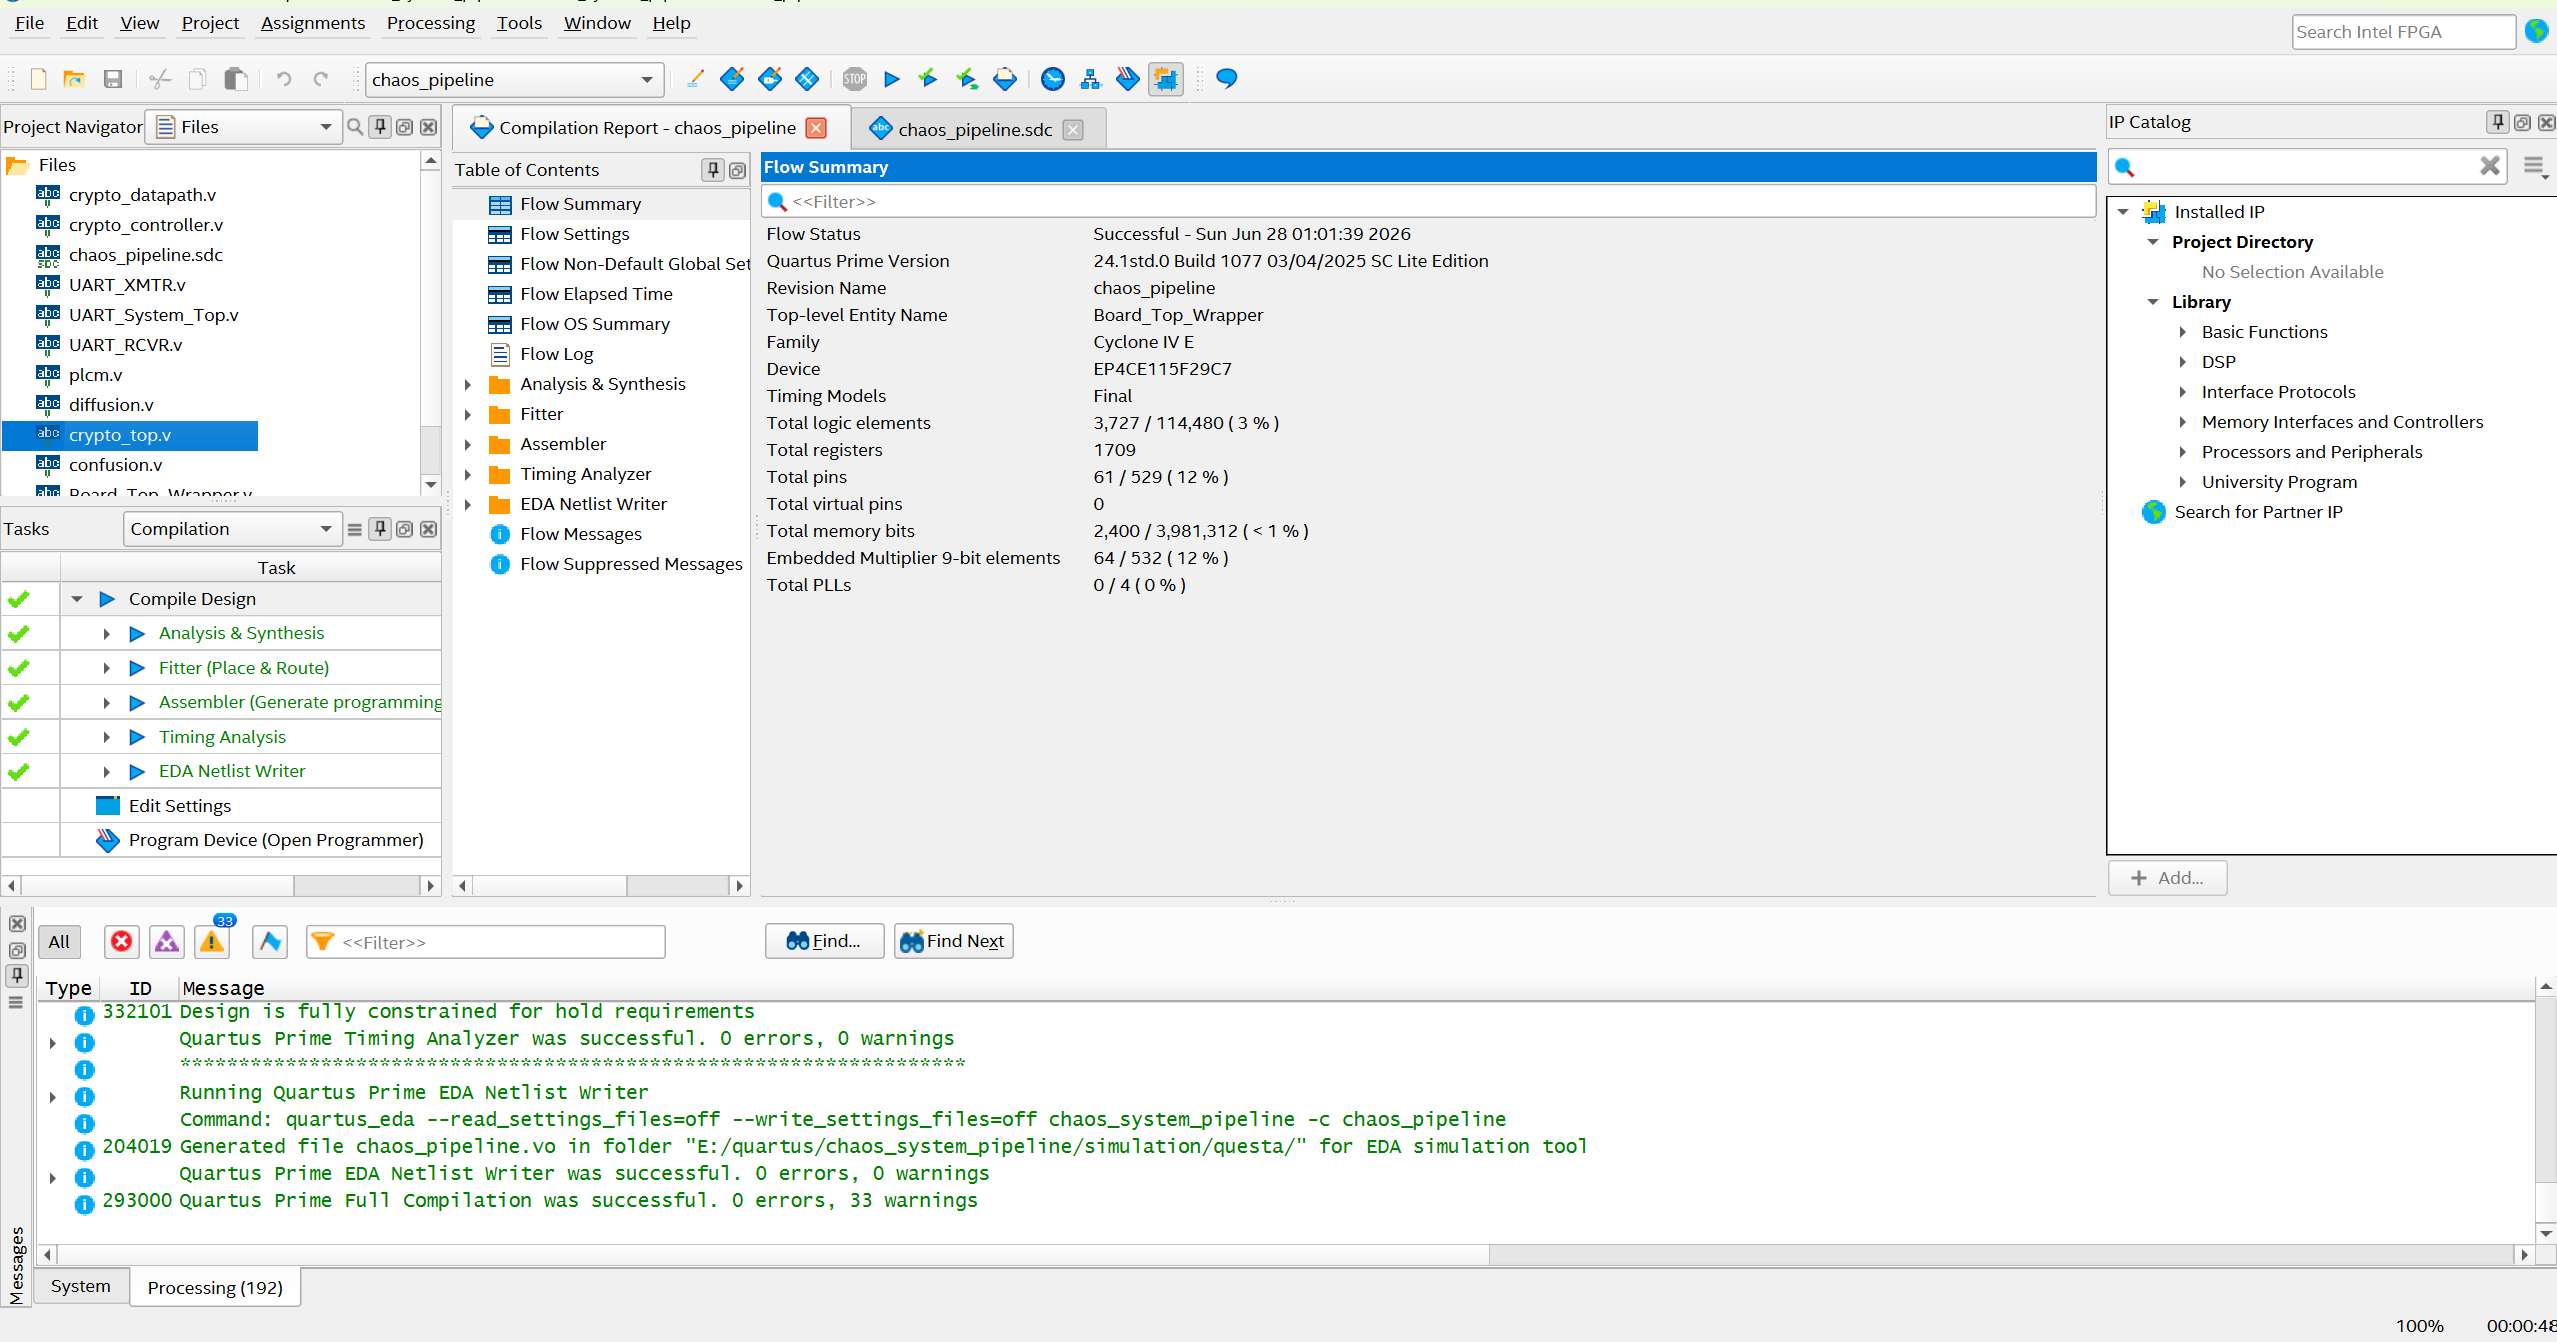
\includegraphics[width=1\textwidth]{Figures/fpga_imp.png}
	\caption{Kết quả tổng hợp thiết kế trên phần mềm Quartus Prime}
	\label{fig:quartus_summary}
\end{figure}

\begin{table}[H]
	\centering
	\caption{Tổng hợp tài nguyên sử dụng sau biên dịch (Dữ liệu tham khảo)}
	\label{tab:resource_usage}
	\renewcommand{\arraystretch}{1.4}
	\begin{tabular}{|l|l|l|}
		\hline
		\textbf{Tài nguyên} & \textbf{Sử dụng / Khả dụng} & \textbf{Tỷ lệ} \\ \hline
		Logic elements & 3 727 / 114 480 & $\sim 3\%$ \\ \hline 
		Registers & 1 709 & -- \\ \hline 
		Pins & 61 / 529 & $\sim 12\%$ \\ \hline
		Memory bits & 2 400 / 3 981 312 & $< 1\%$ \\ \hline 
		Embedded multiplier 9-bit & 64 / 532 & $\sim 12\%$ \\ \hline 
	\end{tabular}
\end{table}

Nhằm đảm bảo tính ổn định của mạch khi vận hành ở xung nhịp cao, hệ thống sử dụng file ràng buộc thời gian để ấn định tần số hoạt động mục tiêu của đồng hồ là 50 MHz. Báo cáo phân tích định thời xác nhận thiết kế vượt qua mọi bài kiểm tra khắt khe, với tần số hoạt động tối đa của mạch đạt 56.87 MHz. Điều này chứng minh các đường trễ tới hạn bên trong kiến trúc máy trạng thái và các đường ống tính toán đã được phân mảnh và tối ưu hóa hiệu quả.

\subsection{Gán chân và thực nghiệm trên FPGA}

Trong bước triển khai cuối cùng, các tín hiệu vào ra của khối thiết kế tổng được gán với các chân cắm vật lý trên bo mạch bằng giao diện Pin Planner. Các tín hiệu cần gán bao gồm nguồn xung nhịp chính, nút nhấn đặt lại hệ thống, công tắc gạt để chọn chế độ mã hóa hoặc giải mã, các chân truyền nhận nối tiếp TTL và nhóm tín hiệu điều khiển trực tiếp 8 LED 7 thanh.

\begin{figure}[H]
	\centering
	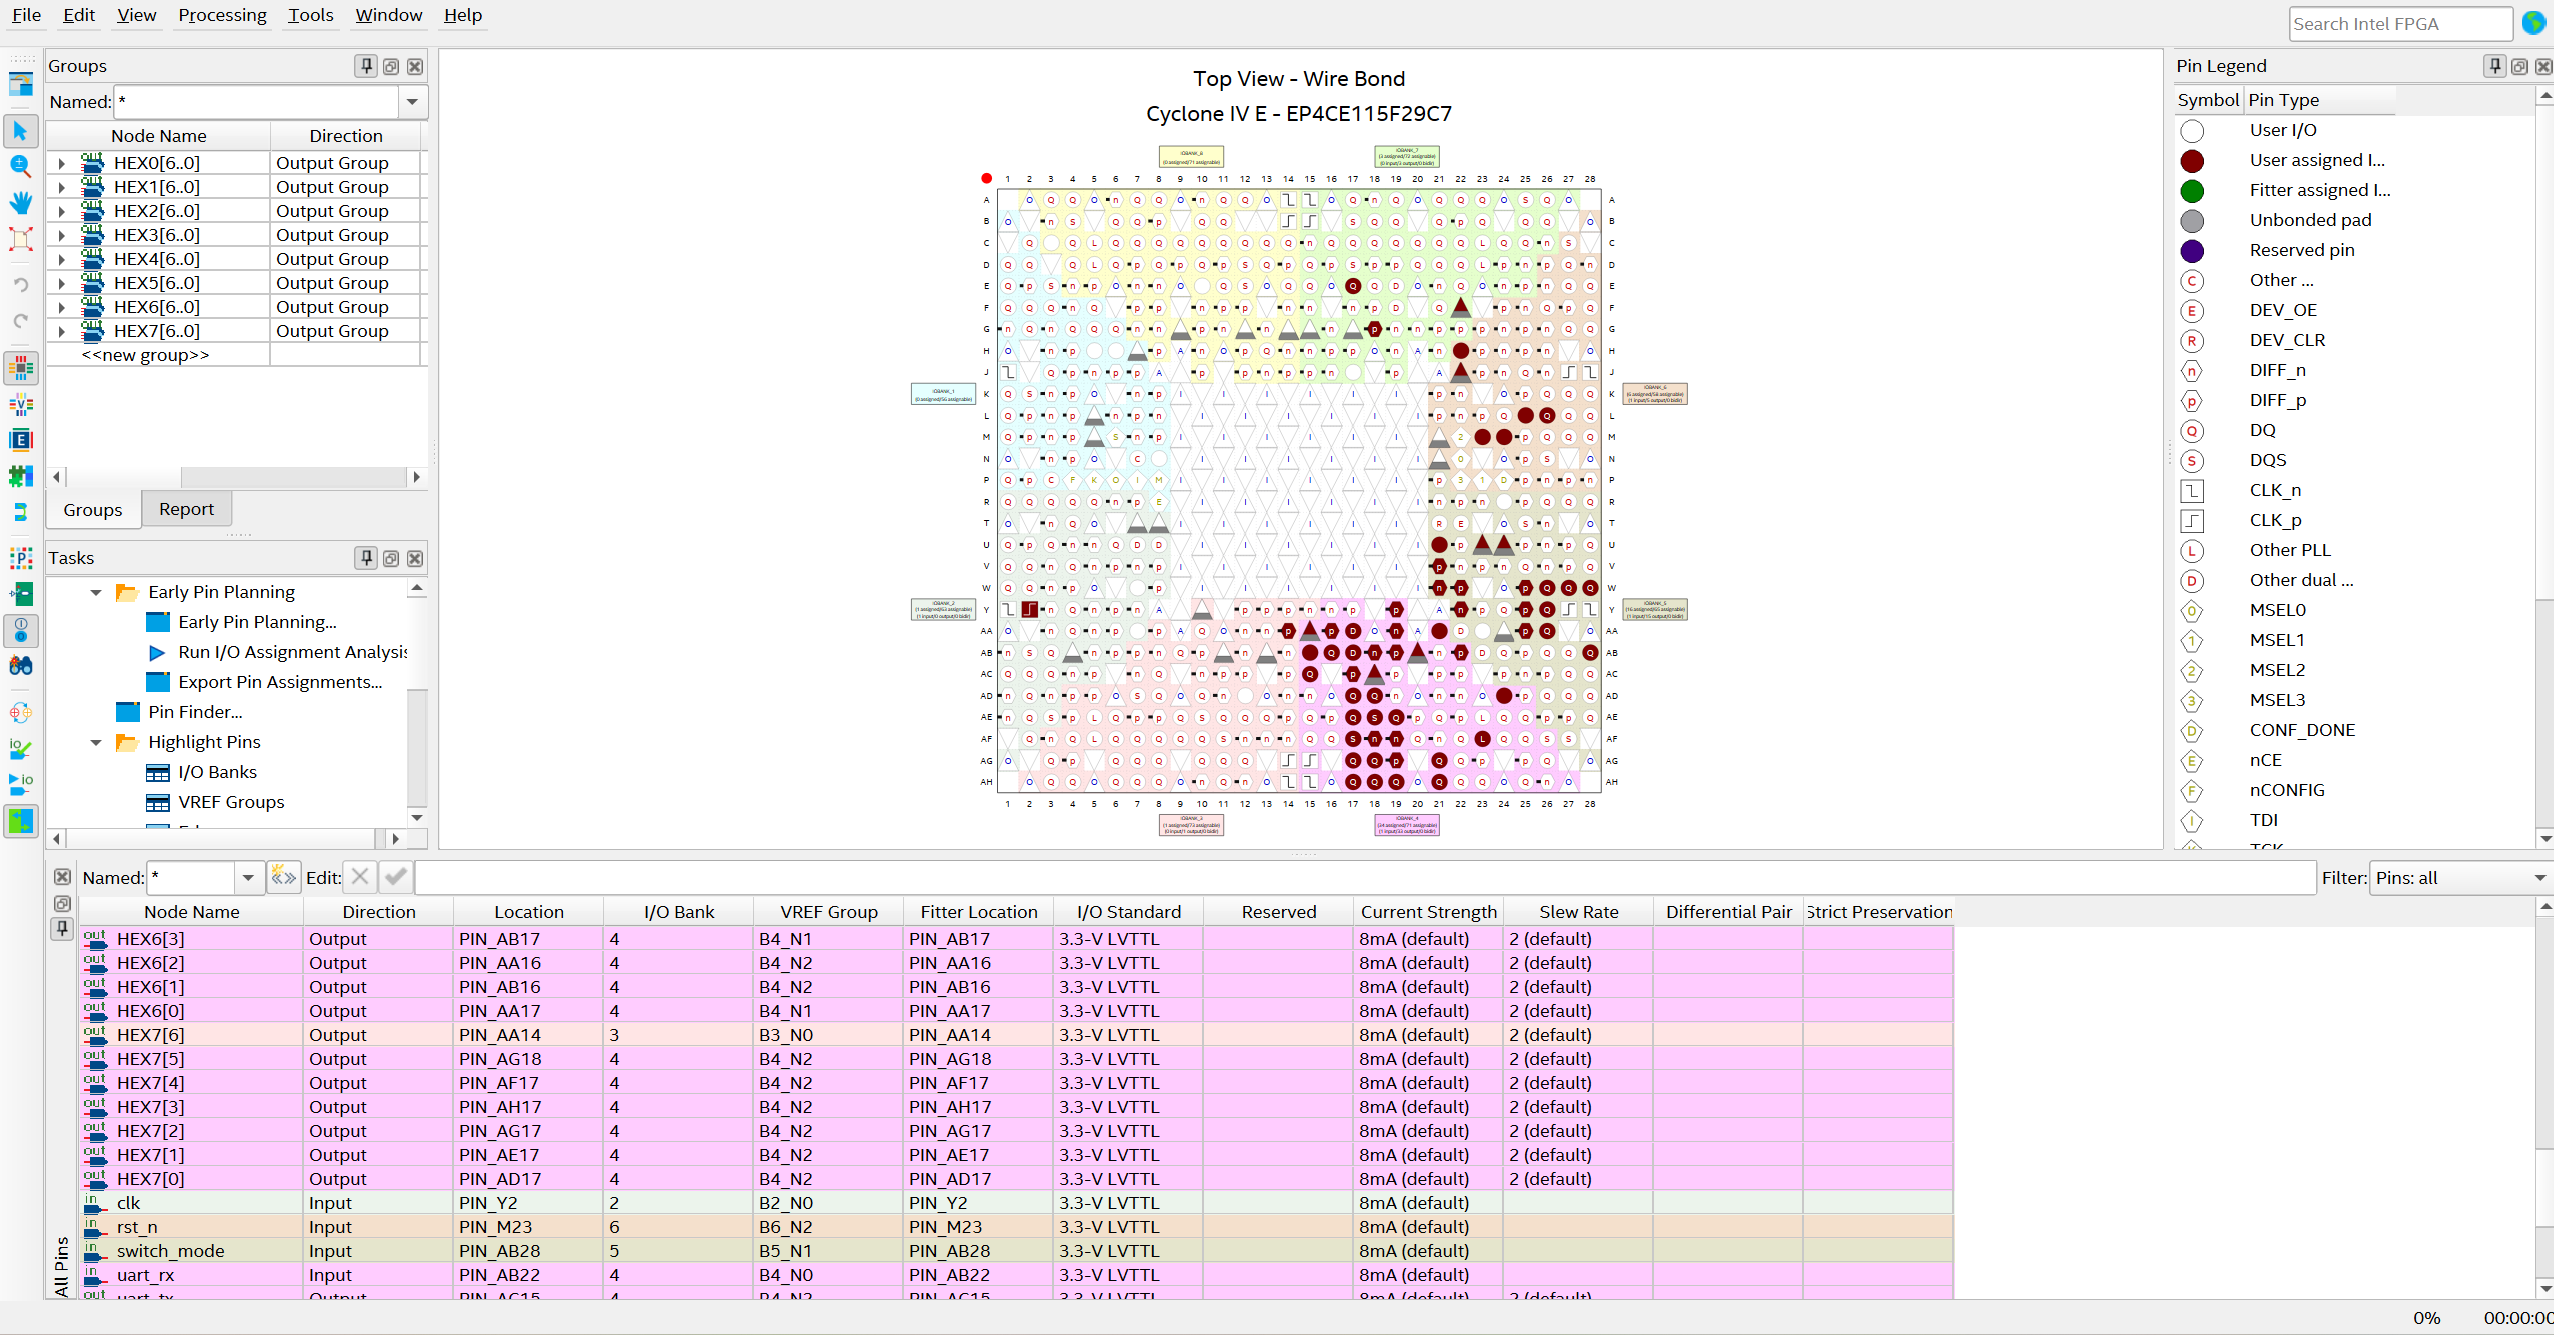
\includegraphics[width=1\textwidth]{Figures/pin.png}
	\caption{Gán chân thiết kế trên giao diện Pin Planner}
	\label{fig:pin_planner}
\end{figure}

\begin{table}[H]
	\centering
	\caption{Sơ đồ gán chân vật lý của thiết kế trên bo mạch DE2-115}
	\label{tab:pin_assignment}
	\renewcommand{\arraystretch}{1.4}
	\begin{tabular}{|l|l|l|p{5.5cm}|}
		\hline
		\textbf{Tín hiệu} & \textbf{Hướng} & \textbf{Chân FPGA} & \textbf{Chức năng} \\ \hline
		\texttt{clk} & Input & PIN\_Y2 & Nguồn xung nhịp 50 MHz. \\ \hline
		\texttt{rst\_n} & Input & PIN\_M23 & Nút nhấn khởi động lại hệ thống. \\ \hline
		\texttt{switch\_mode} & Input & PIN\_AB28 & Công tắc gạt chọn Mã hóa (0) hoặc Giải mã (1). \\ \hline
		\texttt{uart\_rx} & Input & PIN\_AB22 & Nhận luồng dữ liệu từ máy tính. \\ \hline
		\texttt{uart\_tx} & Output & PIN\_AC15 & Xuất luồng kết quả về lại máy tính. \\ \hline
		\texttt{HEX0} -- \texttt{HEX7} & Output & Nhiều chân & Điều khiển LED 7 thanh hiển thị số chu kỳ. \\ \hline
	\end{tabular}
\end{table}

Tệp tin cấu hình thu được sau khi biên dịch được nạp trực tiếp xuống phần cứng thông qua bộ nạp. Quá trình thực nghiệm được tiến hành bằng cách kích hoạt chương trình Python trên máy tính để bơm dữ liệu vào hệ thống. Hình \ref{fig:real_fpga} minh họa bo mạch đang trong quá trình thực thi thuật toán theo thời gian thực, với kết quả hiển thị trên phần mềm máy tính hoàn toàn khớp với kỳ vọng. Cùng lúc đó, số lượng chu kỳ xung nhịp được đếm bằng phần cứng hiện rõ trên dàn LED, phản ánh chân thực tốc độ và hiệu năng của lõi mật mã được thiết kế.

\begin{figure}[H]
	\centering
	% [!CHÚ Ý CHÈN ẢNH THẬT!] Chèn ảnh chụp FPGA đang chạy có hiện số trên LED 7 thanh vào đây
	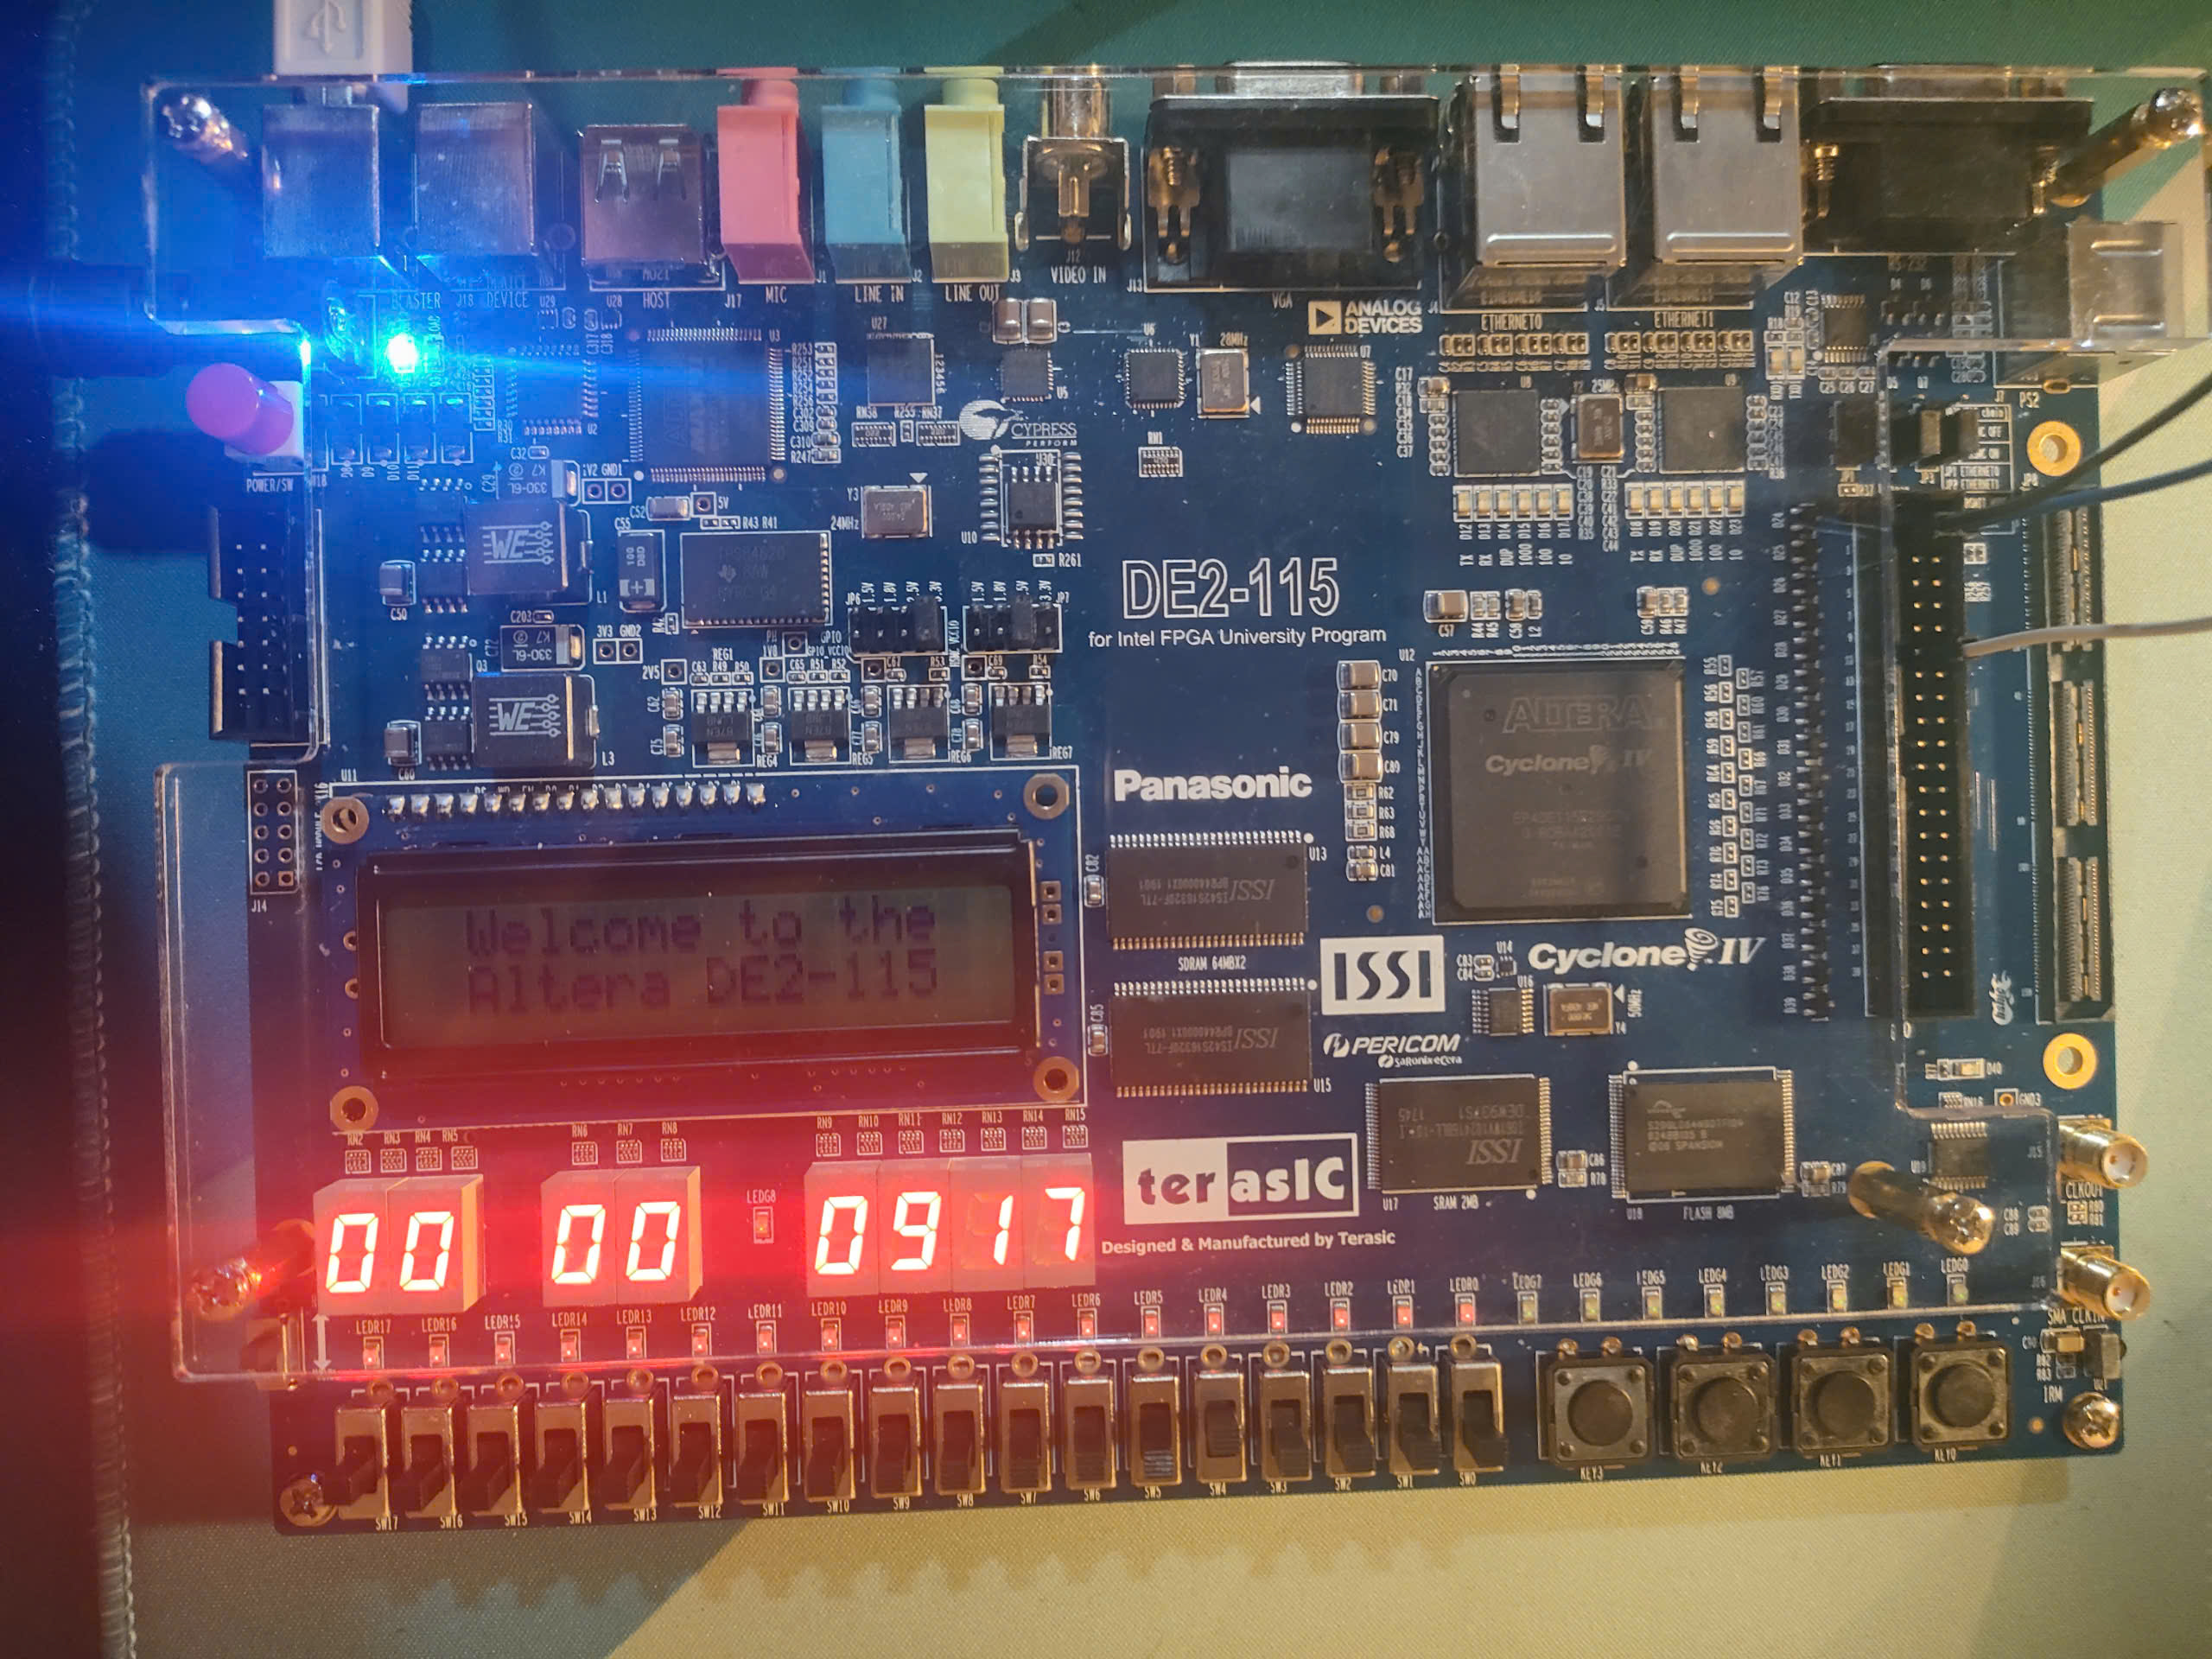
\includegraphics[width=0.6\textwidth]{Figures/100.jpg} 
%	\vspace{5cm} % Xóa dòng vspace này khi đã chèn ảnh
	\caption{Hình ảnh thực nghiệm hệ thống mã hóa hoạt động trên bo mạch DE2-115}
	\label{fig:real_fpga}
\end{figure}

\subsection{Tổng kết chương 9}

Chương 5 đã hiện thực hóa thành công mảnh ghép cuối cùng của đồ án, chuyển đổi thiết kế lý thuyết thành một lõi phần cứng vật lý có khả năng hoạt động độc lập. Bằng việc xây dựng khối bao bọc điều phối thông minh kết hợp cùng bộ đếm chu kỳ, hệ thống đã chứng minh được tính đồng bộ cao trong quá trình giao tiếp đa tốc độ với máy tính thông qua kịch bản phần mềm Python. Mức tiêu thụ tài nguyên cực kỳ khiêm tốn cùng tần số hoạt động đạt yêu cầu trên bo mạch FPGA Cyclone IV đã tái khẳng định tiềm năng ứng dụng thực tế của kiến trúc. Những kết quả thực nghiệm trực quan trên thiết bị vật lý này là minh chứng rõ nét nhất cho tính đúng đắn của toàn bộ quy trình thiết kế video được thực hiện xuyên suốt đồ án.

\clearpage